\section{Methods for Markov Chains}\label{m:sec:methods}

The same stochastic process can be analysed at several levels.  Transition
matrices and generators describe the full law, first-step equations isolate a
particular hitting event, and moments compress the law into summary quantities.
Generating functions occupy the useful middle ground: they retain enough of the
distribution to turn discrete branching into iteration and continuous-time master
equations into PDEs.  The methods are ordered below by the clock on which the
process evolves.

\subsection{Discrete-Time Methods}\label{m:sec:discrete-methods}

For a non-negative integer-valued random variable $X$, its probability generating
function is
\begin{equation}
  \phi(z)=\ex{z^X}=\sum_{k\geq0}\pr{X=k}z^k.
  \label{m:eq:pgfdef}
\end{equation}
Its coefficients determine the distribution, while derivatives at $z=1$ give
factorial moments.  For branching, the more important property is structural:
independent sums become products and a random sum becomes a composition.  The
Galton--Watson recursion \cref{m:eq:gwrecursion} therefore reduces to the
one-dimensional iteration \cref{m:eq:gw-pgf-iteration}.

First-step analysis provides the corresponding local method.  Conditioning on the
first transition makes the same unknown quantity reappear from the new state.  In
the binary process, the founder either leaves no offspring or begins two
independent lineages, giving \cref{m:eq:SnIter} directly.  The map itself is
elementary to iterate, although its late-time matching constant requires a more
specialised analysis.

For $p<\tfrac12$, the survival probabilities tend to zero and obey
\begin{equation}
  S_n\sim A(p)(2p)^n,
  \qquad
  A(p)=\lim_{n\to\infty}\frac{S_n}{(2p)^n}.
  \label{m:eq:lateS}
\end{equation}
Since $\ex{Z_n}=(2p)^n$ and $Z_n=0$ on extinction,
\begin{equation}
  \ex{Z_n\mid Z_n>0}
  =\frac{(2p)^n}{S_n}
  \longrightarrow\frac{1}{A(p)}.
  \label{m:eq:discrete-conditional-mean}
\end{equation}
Equations \cref{m:eq:lateS,m:eq:discrete-conditional-mean} provide the complete
discrete-$A(p)$ interface needed here.  \ChA{} develops the product and series
representations, bounds, near-critical asymptotics and Koenigs-function methods;
that deeper theory is not repeated in this chapter.

The same conditioning has a finite limiting variance.  A second-moment recursion
for the binary process gives
\begin{equation}
  \var{Z_n\mid Z_n>0}\longrightarrow
  \frac{1}{A(p)}\left(1+\frac{1}{1-2p}\right)
  -\frac{1}{A(p)^2}.
  \label{m:eq:discrete-conditional-variance}
\end{equation}
This is still only a light use of $A(p)$: the moment calculation treats it as the
normalising constant already defined in \cref{m:eq:lateS}.  The full derivation is
given in \cref{m:app:conditional-variance}; its product, series and analytic
structure remain exclusively in \ChA.

\subsection{Continuous-Time Methods}\label{m:sec:continuous-methods}

The generator of a continuous-time chain supports complementary forward and
backward viewpoints.  The forward equation propagates a distribution, making it
the natural starting point for master equations and generating functions.  The
backward equation instead fixes a terminal state or observable and asks how its
value depends on the initial state, which is particularly efficient for hitting
and extinction probabilities and for transforms of hitting times.

For a time-homogeneous chain, the transition matrices form a semigroup:
\begin{equation}
  P(s+t)=P(s)P(t),
  \qquad P(0)=I.
  \label{m:eq:ctmc-semigroup}
\end{equation}
The generator is the infinitesimal derivative at zero,
\begin{equation}
  Q=\lim_{h\downarrow0}\frac{P(h)-I}{h},
  \qquad P(h)=I+hQ+o(h).
  \label{m:eq:generator-semigroup-limit}
\end{equation}
Inserting the short-time expansion into the semigroup relation in its two
equivalent orders explains the two Kolmogorov equations.  From
$P(t+h)=P(t)P(h)$, the short interval acts at the end of the path and gives the
forward equation.  From $P(t+h)=P(h)P(t)$, it acts at the beginning and gives the
backward equation.  The matrices coincide as derivatives of the same semigroup,
but their componentwise interpretations differ because one resolves the final
state and the other resolves the first jump from the initial state.

This distinction prevents a common notational error.  With row distributions,
$p(t)=p(0)P(t)$ and hence $p'(t)=p(t)Q$.  A function of the initial state is
naturally a column vector, on which the generator acts from the left.  The same
entries $q_{ij}$ appear in both calculations, but the object being evolved fixes
the multiplication order.  All subsequent equations use this convention.

\subsubsection{Backward equations}\label{m:sec:backward-equations}

In matrix notation the two Kolmogorov equations are
\begin{equation}
  \frac{\dd P(t)}{\dd t}=P(t)Q,
  \qquad
  \frac{\dd P(t)}{\dd t}=QP(t),
  \label{m:eq:kolmogorov-pair}
\end{equation}
with the order of multiplication distinguishing forward propagation from backward
dependence on the initial state.  For a branching process the backward equation
can close nonlinearly because independent descendants contribute copies of the same
one-ancestor quantity.  For example, the PGF $F(x,t)$ of an interior linear
birth--death process started from one individual satisfies
\begin{equation}
  \pddt{F}=\lambda F^2-(\lambda+\mu)F+\mu,
  \qquad F(x,0)=x.
  \label{m:eq:bd-backward}
\end{equation}
Indeed, during a short initial interval of length $h$, the founder dies, gives
birth, or experiences no event with probabilities $\mu h$, $\lambda h$ and
$1-(\lambda+\mu)h$, up to $o(h)$.  After a birth, two independent descendant
families remain for the residual time.  The branching property therefore gives
\begin{equation}
  F(x,t+h)=\mu h+\lambda hF(x,t)^2
  +\{1-(\lambda+\mu)h\}F(x,t)+o(h),
  \label{m:eq:bd-backward-step}
\end{equation}
and division by $h$ recovers \cref{m:eq:bd-backward}.  The calculation exposes
why the forward equation is linear in the state probabilities while the backward
one-founder equation is nonlinear in the PGF.

The generator, master equation and first-step calculation are therefore three
representations of the same local transition rules.

\subsubsection{Generator identities and observables}
\label{m:sec:generator-observables}

The generator also evolves observables without first reconstructing the entire
distribution.  For a suitable function $f$ and a non-explosive chain,
\begin{equation}
  \frac{\dd}{\dd t}\ex{f(X_t)}=\ex{(\mathcal Lf)(X_t)}.
  \label{m:eq:generator-expectation}
\end{equation}
This is the expectation form of the backward equation.  It follows by applying
the infinitesimal transition rule over an interval of length $h$, conditioning on
$X_t$, and dividing the expected increment by $h$.  For the linear birth--death
generator \cref{m:eq:bd-generator-action}, the choices $f(n)=n$ and
$f(n)=n(n-1)$ give
\begin{align}
  (\mathcal Lf)(n)&=(\lambda-\mu)n,
  && f(n)=n,\label{m:eq:generator-first-action}\\
  (\mathcal Lf)(n)&=2(\lambda-\mu)n(n-1)+2\lambda n,
  && f(n)=n(n-1).
  \label{m:eq:generator-second-action}
\end{align}
Thus the same moment equations can be obtained either from generator algebra or
by differentiating the generating-function PDE.  The former is usually quicker
for a small number of moments; the latter keeps the whole hierarchy and remains
available when a distributional answer is required.

\subsubsection{Mean population size}\label{m:sec:ct-mean}

For the linear birth--death chain, each individual contributes births at rate
$\lambda$ and deaths at rate $\mu$.  Taking the first moment of the master equation,
or differentiating \cref{m:eq:bdpde} once at $z=1$, gives
\begin{equation}
  \frac{\dd}{\dd t}\ex{X_t}=(\lambda-\mu)\ex{X_t},
  \qquad
  \ex{X_t}=N\ee^{(\lambda-\mu)t}.
  \label{m:eq:bdmean}
\end{equation}
The sign of $\lambda-\mu$ separates subcritical, critical and supercritical mean
behaviour.  This division is useful but incomplete, because the mean alone does not
determine extinction or the shape of the state distribution.

\subsubsection{Variance and higher moments}\label{m:sec:ct-higher-moments}

Generating functions organise the moment hierarchy.  At any fixed $t$,
\begin{equation}
  \left.\pdd{G}{z}\right|_{z=1}=\ex{X_t},
  \qquad
  \left.\frac{\partial^2G}{\partial z^2}\right|_{z=1}
  =\ex{X_t(X_t-1)},
  \label{m:eq:pgf-moments}
\end{equation}
so the first two derivatives determine the variance and repeated differentiation
gives higher factorial moments.  Differentiating the PDE \cref{m:eq:bdpde} in this
way replaces the infinite probability system by ordinary differential equations
for the moments.  If
\[
  M_1(t)=\left.G_z\right|_{z=1},
  \qquad
  M_2(t)=\left.G_{zz}\right|_{z=1},
\]
then differentiating once and twice before setting $z=1$ shows explicitly that
the first moment closes and that the second factorial moment is driven only by
the first two:
\begin{align}
  M_1'(t)&=(\lambda-\mu)M_1(t),
  \label{m:eq:ct-first-factorial}\\
  M_2'(t)&=2(\lambda-\mu)M_2(t)+2\lambda M_1(t).
  \label{m:eq:ct-second-factorial}
\end{align}
The variance is $M_2+M_1-M_1^2$.  Further differentiation produces the same
triangular pattern: the equation for the $r$th factorial moment involves moments
of order at most $r$.  This hierarchy is often preferable to solving for every
$p_n(t)$ when only a few population summaries are required.

The initial conditions are inherited from the starting population.  If $X_0=N$
deterministically, then $M_1(0)=N$ and $M_2(0)=N(N-1)$.  Consequently
\cref{m:eq:ct-first-factorial,m:eq:ct-second-factorial} form a closed, sequential
calculation: solve for $M_1$, insert that result into the linear equation for
$M_2$, and only then convert factorial moments to the ordinary variance.  This
order avoids expanding the master equation term by term and makes clear which
parts of the calculation depend on the linear per-capita assumption.  Nonlinear
rates generally introduce expectations of higher powers and destroy this simple
closure.

\subsubsection{Hitting probabilities}\label{m:sec:hitting-probabilities}

When the target is the probability of reaching one set before another, the full
time-dependent law is usually unnecessary.  Conditioning on the first exponential
clock to ring gives a linear system for the desired probabilities over the
transient states.  Equivalently, the unknown function is harmonic for the killed
generator in the interior, with boundary values fixed on the target sets.  This
viewpoint covers ordinary extinction at $0$ and, for \cref{m:eq:bdcrates}, the
competing event of reaching $\dagger$.

More precisely, let $A$ and $B$ be disjoint absorbing target sets and put
$h_i=\mathbb P_i(\tau_A<\tau_B)$.  Conditioning on the first jump from a transient
state $i$ yields
\begin{equation}
  h_i=\sum_{j\neq i}\frac{q_{ij}}{q_i}h_j,
  \qquad\text{or equivalently}\qquad
  (Qh)_i=0,
  \label{m:eq:hitting-harmonic}
\end{equation}
with boundary data $h=1$ on $A$ and $h=0$ on $B$.  Expected hitting times obey
the inhomogeneous companion equation
\begin{equation}
  (Qv)_i=-1
  \label{m:eq:mean-hitting-time}
\end{equation}
on the transient states, with $v=0$ on the target.  These equations separate the
eventual destination from the holding times: jump probabilities determine
\cref{m:eq:hitting-harmonic}, while the rates also enter
\cref{m:eq:mean-hitting-time} through the mean wait $1/q_i$.

The same construction handles transforms of hitting times.  If
$w_i(s)=\mathbb E_i[\exp(-s\tau_A);\tau_A<\tau_B]$, the first holding time
contributes an additional discount and the interior equation becomes
\begin{equation}
  (Qw)_i=s w_i,
  \label{m:eq:hitting-laplace}
\end{equation}
with $w=1$ on $A$ and $w=0$ on $B$.  Differentiating at $s=0$, when justified,
returns time moments.  Probability, mean time and transform are therefore not
separate tricks: they are the homogeneous, Poisson and resolvent versions of the
same killed-generator boundary problem.

\subsubsection{Extinction probabilities}\label{m:sec:extinction-probabilities}

For the linear birth--death chain started from $N$ individuals, the characteristic
solution of \cref{m:eq:bdpde} is \cite{Kendall1948}
\begin{equation}
  G(z,t)=
  \left[
  \frac{\mu(1-z)-(\mu-\lambda z)\ee^{-(\lambda-\mu)t}}
       {\lambda(1-z)-(\mu-\lambda z)\ee^{-(\lambda-\mu)t}}
  \right]^N,
  \qquad \lambda\neq\mu.
  \label{m:eq:bdsolution}
\end{equation}
The same extinction law follows directly from the backward equation.  Setting
$q(t)=F(0,t)$ in \cref{m:eq:bd-backward} gives
\begin{equation}
  q'(t)=\lambda q(t)^2-(\lambda+\mu)q(t)+\mu,
  \qquad q(0)=0.
  \label{m:eq:bd-extinction-riccati}
\end{equation}
For $\lambda\neq\mu$ the right-hand side factorises as
$\lambda(q-1)(q-\mu/\lambda)$ and separates; at criticality it becomes
$\lambda(q-1)^2$.  Independence of the $N$ founder families then raises the
one-founder extinction probability to the $N$th power.

The forward PGF gives the same answer through characteristics.  Writing
$b(z)=(\lambda z-\mu)(z-1)$, \cref{m:eq:bdpde} is
$G_t-b(z)G_z=0$.  Along a characteristic,
\begin{equation}
  \frac{\dd z}{\dd t}=-b(z),
  \qquad
  \frac{\dd G}{\dd t}=0.
  \label{m:eq:bd-characteristic-system}
\end{equation}
For $\lambda\neq\mu$, separation gives the invariant relation
\begin{equation}
  \frac{z(t)-1}{\lambda z(t)-\mu}
  =\ee^{(\mu-\lambda)t}
   \frac{z(0)-1}{\lambda z(0)-\mu}.
  \label{m:eq:bd-characteristic-invariant}
\end{equation}
The initial condition is $G(z,0)=z^N$, so one solves
\cref{m:eq:bd-characteristic-invariant} for the foot $z(0)$ of the
characteristic and raises that value to the $N$th power.  This inversion produces
\cref{m:eq:bdsolution}.  At $\lambda=\mu$ the two roots coalesce; integrating
the resulting repeated-root equation gives the second line of
\cref{m:eq:p0t} directly.

Setting $z=0$ extracts the probability of extinction by time $t$:
\begin{equation}
  p_0(t)=
  \begin{cases}
  \displaystyle
  \left[
  \frac{\mu-\mu\ee^{(\mu-\lambda)t}}
       {\lambda-\mu\ee^{(\mu-\lambda)t}}
  \right]^N,&\lambda\neq\mu,\\[12pt]
  \displaystyle\left(\frac{\lambda t}{1+\lambda t}\right)^N,
       &\lambda=\mu.
  \end{cases}
  \label{m:eq:p0t}
\end{equation}
Letting $t\to\infty$ shows that extinction is certain when $\lambda\leq\mu$ and
has probability $(\mu/\lambda)^N$ when $\lambda>\mu$.

The three regimes differ even when ultimate extinction is certain.  In the
subcritical case the survival probability has an exponential tail.  At
criticality, \cref{m:eq:p0t} gives
\begin{equation}
  \pr{X_t>0\mid X_0=1}=\frac{1}{1+\lambda t},
  \label{m:eq:ct-critical-survival}
\end{equation}
the continuous-time counterpart of the $n^{-1}$ decay in
\cref{m:eq:critical-summary}.  In the supercritical case a positive fraction of
paths escape extinction altogether.

These results also illustrate why an unconditional mean can be misleading near
absorption.  In the subcritical regime almost all paths are eventually at zero,
yet the few paths still alive may contain several individuals.  At criticality
the mean remains constant while the survival probability decays as $t^{-1}$, so
the surviving population must grow on the reciprocal scale.  Conditional means
make that balancing mechanism explicit.

\subsubsection{Conditional means}\label{m:sec:conditional-means}

Conditioning on non-extinction separates the transient population from the mass
already absorbed at zero.  For one initial individual in the subcritical case
$\mu>\lambda$, \cref{m:eq:p0t} gives
\begin{equation}
  S(t)=\pr{X_t>0}
  =\frac{\lambda-\mu}{\lambda-\mu\ee^{(\mu-\lambda)t}},
  \label{m:eq:ct-survival}
\end{equation}
whereas \cref{m:eq:bdmean} gives
$\ex{X_t}=\ee^{(\lambda-\mu)t}$.  Since $X_t=0$ on extinction,
\begin{equation}
  \ex{X_t\mid X_t>0}
  =\frac{\ex{X_t}}{S(t)}
  =\frac{\lambda\ee^{(\lambda-\mu)t}-\mu}{\lambda-\mu}
  \longrightarrow\frac{\mu}{\mu-\lambda}.
  \label{m:eq:ct-conditional-mean}
\end{equation}

The comparison with the discrete binary process uses the competing-clock identity
\cref{m:eq:competing-clocks}.  If the birth and death clocks have rates $\lambda$
and $\mu$, then the probability that birth occurs first is
\begin{equation}
  p=\frac{\lambda}{\lambda+\mu},
  \qquad \frac{\lambda}{\mu}=\frac{p}{1-p}.
  \label{m:eq:rate-match}
\end{equation}
Substitution into \cref{m:eq:ct-conditional-mean} gives
\begin{equation}
  \lim_{t\to\infty}\ex{X_t\mid X_t>0}
  =\frac{1-p}{1-2p}=\frac{1}{\Ac(p)},
  \qquad
  \boxed{\Ac(p)=\frac{1-2p}{1-p}}.
  \label{m:eq:Acts}
\end{equation}

\begin{figure}[tbp]
  \centering
  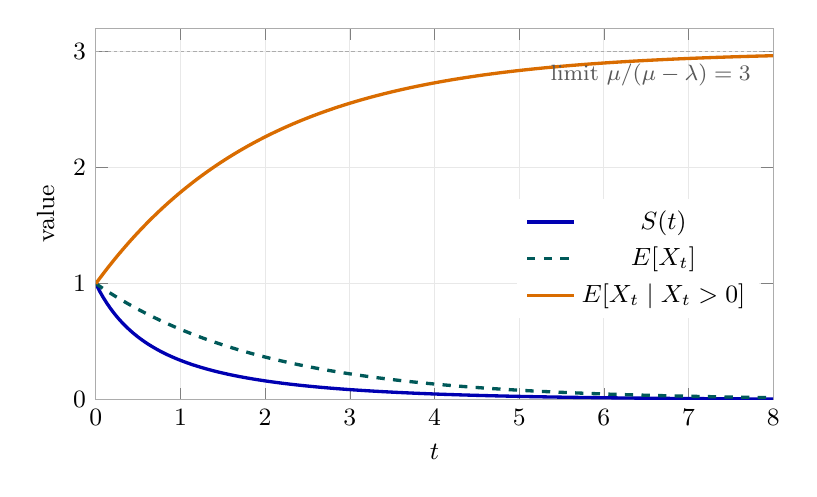
\begin{tikzpicture}
    \begin{axis}[
      width=0.84\textwidth,
      height=6.3cm,
      domain=0:8,
      samples=180,
      xmin=0, xmax=8,
      ymin=0, ymax=3.2,
      xlabel={$t$},
      ylabel={value},
      grid=major,
      grid style={draw=gray!18},
      axis line style={draw=gray!65},
      tick label style={font=\small},
      label style={font=\small},
      legend style={font=\small, draw=none, fill=white, at={(0.98,0.38)},
        anchor=east, row sep=1pt},
      every axis plot/.append style={very thick}
    ]
      \addplot[blue!70!black] {0.5/(1.5*exp(0.5*x)-1)};
      \addlegendentry{$S(t)$}
      \addplot[teal!70!black, dashed] {exp(-0.5*x)};
      \addlegendentry{$\mathbb E[X_t]$}
      \addplot[orange!85!black] {3-2*exp(-0.5*x)};
      \addlegendentry{$\mathbb E[X_t\mid X_t>0]$}
      \addplot[gray!65, densely dotted, thin] coordinates {(0,3) (8,3)};
      \node[anchor=north east, font=\footnotesize, text=gray!70!black]
        at (axis cs:7.85,2.98) {limit $\mu/(\mu-\lambda)=3$};
    \end{axis}
  \end{tikzpicture}
  \caption{Survival probability, unconditional mean and conditional mean for
  the subcritical linear birth--death process with $\lambda=1$, $\mu=3/2$ and
  $X_0=1$.  Although both survival and the unconditional mean decay, the mean
  among surviving realisations approaches a non-zero limit.}
  \label{m:fig:ct-conditioning}
\end{figure}

The continuous-time conditional-mean constant is therefore elementary.  Its
discrete counterpart is the lightly defined $A(p)$ of \cref{m:eq:lateS}, whose
reciprocal is the conditional mean.  The constants are not identical; their exact
comparison and the obstruction arising from discrete functional iteration are
developed in \ChA.

For completeness, at criticality the same division by
\cref{m:eq:ct-critical-survival} gives
\begin{equation}
  \ex{X_t\mid X_t>0}=1+\lambda t,
  \label{m:eq:ct-critical-conditional-mean}
\end{equation}
so there is no stationary conditional mean at the threshold.  For fixed
$N>1$ in the subcritical regime, both the mean and the late survival probability
acquire the same leading factor $N$; their ratio therefore has the same limit
$1/\Ac(p)$ as the one-founder process.

\subsubsection{Conditioning and killed semigroups}
\label{m:sec:conditioning-killed-semigroups}

Conditional means are one projection of a broader construction.  Let $T$ be an
absorption time and let $K$ be the generator restricted to the transient states.
If the initial distribution on those states is the row vector $\gamma$, then the
unconditional transient law is
\begin{equation}
  \gamma\ee^{tK}.
  \label{m:eq:killed-semigroup-law}
\end{equation}
Its total mass is the survival probability
$\gamma\ee^{tK}\mathbf 1$.  Normalising by that mass gives the law seen among
realisations that have not yet been absorbed:
\begin{equation}
  \mathbb P_\gamma(X_t=j\mid T>t)
  =\frac{(\gamma\ee^{tK})_j}
         {\gamma\ee^{tK}\mathbf 1}.
  \label{m:eq:conditioned-killed-law}
\end{equation}
\begin{figure}[H]
  \centering
  \begin{tikzpicture}[
    font=\small,
    box/.style={draw=blue!60!black, fill=blue!6, rounded corners=3pt,
      minimum height=13mm, text width=32mm, align=center},
    start/.style={draw=gray!65, fill=gray!7, rounded corners=3pt,
      minimum height=13mm, text width=24mm, align=center},
    conditioned/.style={draw=teal!65!black, fill=teal!7, rounded corners=3pt,
      minimum height=13mm, text width=39mm, align=center},
    absorbed/.style={draw=red!65!black, fill=red!6, rounded corners=3pt,
      minimum height=14mm, text width=59mm, align=center},
    flow/.style={-{Stealth[length=2.3mm]}, semithick, draw=gray!75!black},
    loss/.style={-{Stealth[length=2.3mm]}, semithick, draw=red!70!black}
  ]
    \node[start] (initial) {initial law\\$\gamma$};
    \node[box, right=10mm of initial] (killed)
      {killed evolution\\$\gamma\ee^{tK}$\\[-1pt]
       \footnotesize mass $s(t)=\gamma\ee^{tK}\mathbf 1$};
    \node[conditioned, right=12mm of killed] (conditional)
      {law given survival\\[1pt]
       $\displaystyle\frac{\gamma\ee^{tK}}{s(t)}$};
    \node[absorbed, below=14mm of killed] (absorbed)
      {absorbed mass $1-s(t)$\\[-1pt]
       \footnotesize ordinary extinction through state $1$ or\\
       catastrophe from positive states};

    \draw[flow] (initial) -- node[above, font=\footnotesize] {$\ee^{tK}$} (killed);
    \draw[flow] (killed) -- node[above, font=\footnotesize, align=center]
      {renormalise\\by $s(t)$} (conditional);
    \draw[loss] (killed) -- node[right, font=\footnotesize] {lost mass} (absorbed);
    \draw[flow, dashed, teal!70!black] (conditional.south) .. controls +(0,-13mm)
      and +(18mm,0) .. node[below right, font=\footnotesize, align=left]
      {shape is unchanged when\\$\nu K=-\theta\nu$} (conditional.east);
  \end{tikzpicture}
  \caption{Killed evolution and conditioning are distinct operations.  The
  sub-probability law $\gamma\ee^{tK}$ loses mass to absorption; division by its
  surviving mass produces the conditional law.  A quasi-stationary distribution
  retains its shape under this renormalised evolution.}
  \label{m:fig:killed-conditioning-flow}
\end{figure}
Although the unnormalised evolution is linear, this division makes the
conditioned evolution nonlinear.  The numerator loses mass to absorption while
the denominator continually rescales what remains.

A distribution $\nu$ is quasi-stationary when the normalised law in
\cref{m:eq:conditioned-killed-law} equals $\nu$ for every $t$ if it begins from
$\nu$.  The eigenrelation
\begin{equation}
  \nu K=-\theta\nu
  \label{m:eq:qsd-left-eigenvector}
\end{equation}
then gives
$\nu\ee^{tK}=\ee^{-\theta t}\nu$: survival decays exponentially, but the
relative weights of the surviving states do not change.  In the BDC process the
identity for $\theta$ in \cref{m:eq:bdc-qsd-eigenrelation} separates the ordinary
extinction flux through state $1$ from the catastrophe flux across all positive
states.  State-dependent killing changes the eigenvector as well as the decay
rate; a constant killing clock only shifts the eigenvalue.

Quasi-stationarity is useful even when the process is not started from $\nu$.
Under appropriate conditions, the conditional law from a wider class of initial
states converges to a Yaglom limit as $t$ grows \cite{Yaglom1947,Meleard2012,
Collet2013}.  The binary Galton--Watson calculation in
\cref{m:eq:discrete-conditional-mean,m:eq:discrete-conditional-variance}
identifies the first two limiting conditional moments without reproving that
general convergence theorem.  Likewise, the birth--death calculation above
obtains the limiting conditional mean directly from an exact survival law.

This viewpoint clarifies the role of the constants.  The continuous-time model
has an explicit killed evolution, and its limiting conditional mean reduces to
$1/\Ac(p)$.  In discrete time the corresponding normalisation is the late-survival
constant $A(p)$.  \ChA{} studies why functional iteration makes that constant
analytically more difficult.  The present chapter needs only the probabilistic
interface: absorption removes mass, conditioning renormalises the surviving law,
and the reciprocal survival amplitude controls its mean.

\subsubsection*{A method-selection summary}

The methods answer different questions from the same generator.  Their division
of labour for the birth--death example is summarised in
\cref{m:tab:ct-method-summary}.
\begin{table}[H]
  \centering
  \small
  \begin{tabular}{>{\raggedright\arraybackslash}p{0.24\textwidth}
                  >{\raggedright\arraybackslash}p{0.31\textwidth}
                  >{\raggedright\arraybackslash}p{0.32\textwidth}}
    \toprule
    Question & Main object & Governing relation \\
    \midrule
    Full state law & forward probabilities or PGF &
      $p'(t)=p(t)Q$ or \cref{m:eq:bdpde} \\
    Dependence on initial state & backward observable &
      $P'(t)=QP(t)$; one-founder equation \cref{m:eq:bd-backward} \\
    A few summaries & generator applied to observables &
      \cref{m:eq:generator-expectation} and the moment hierarchy \\
    Eventual destination & harmonic boundary problem &
      $Qh=0$ with absorbing boundary values \\
    Time to a target & Poisson or resolvent problem &
      $Qv=-1$ or \cref{m:eq:hitting-laplace} \\
    Law before absorption & killed semigroup and normalisation &
      \cref{m:eq:conditioned-killed-law} \\
    \bottomrule
  \end{tabular}
  \caption{Continuous-time methods organised by the quantity sought.  The
  generator is common to every row; the choice of observable or boundary
  condition determines the calculation.}
  \label{m:tab:ct-method-summary}
\end{table}

\subsection{Method of Characteristics}\label{m:sec:moc}

A first-order generating-function PDE has the schematic form
\[
  a_t\pddt{G}+a_x\pdd{G}{x}+a_y\pdd{G}{y}=bG+c.
\]
The method of characteristics chooses curves in $(x,y,t)$ with tangent vector
$(a_x,a_y,a_t)$.  Along each curve, the chain rule turns the PDE into an ordinary
differential equation for $G$.  The calculation proceeds in three stages: derive
the PDE from the master equation, integrate the characteristic ODEs from a
parametrised initial surface, and invert that parametrisation to recover
$G(x,y,t)$.  The following example carries out all three stages in a case whose
answer can also be obtained from independence.

The initial surface matters.  For an evolution problem it is naturally the plane
$t=0$, parametrised by the remaining generating-function variables.  A point
$(x,y,t)$ is traced backwards along its characteristic until it meets that plane;
the initial PGF then supplies the value carried forward along the same curve.  The
last inversion step is therefore not cosmetic: it identifies which point of the
initial surface feeds the requested point at time $t$.

In practice the calculation is best kept in a fixed order.
\begin{enumerate}[label=\arabic*., leftmargin=2em]
  \item Derive the PGF PDE from the forward equations, displaying at least one
  index shift so that signs and boundary terms can be checked.
  \item Move all derivative terms to one side and read off the characteristic
  vector field.  A consistent sign convention is essential because reversing the
  time component reverses every other characteristic equation.
  \item Parametrise the initial surface and integrate the characteristic ODEs
  with those initial values, retaining the labels of the surface coordinates.
  \item Invert the map from surface coordinates to $(x,y,t)$ before substituting
  the initial PGF.  This is often the longest algebraic step.
  \item Check the initial condition, normalisation at unit PGF arguments, and at
  least one independent moment or finite-state reduction.
\end{enumerate}
These stages separate probabilistic bookkeeping from differential-equation
algebra.  They also locate errors: a failure at $G(1,1,t)=1$ usually points to the
PDE or its signs, whereas a correct PDE but incorrect initial value points to the
characteristic inversion.

\begin{figure}[tbp]
  \centering
  \begin{tikzpicture}[
    font=\small,
    surface/.style={draw=blue!65!black, fill=blue!8, rounded corners=2pt},
    flow/.style={-{Stealth[length=2.3mm]}, very thick, draw=teal!70!black}
  ]
    \draw[surface] (-4.2,-0.45) -- (1.5,-0.45) -- (3.2,0.55) -- (-2.5,0.55) -- cycle;
    \node[blue!60!black] at (-3.15,0.03) {initial surface $t=0$};
    \fill[blue!70!black] (0,0) circle (2pt)
      node[below=4pt] {$(\sigma,\eta,0)$};
    \draw[flow] (0,0) .. controls (0.65,1.1) and (1.8,1.25) .. (2.5,2.15);
    \fill[teal!75!black] (2.5,2.15) circle (2.2pt)
      node[above right=-1pt] {$(x,y,t)$};
    \node[teal!70!black, align=center] at (0.9,1.45)
      {characteristic\\$G$ transported by an ODE};
    \draw[-{Stealth[length=2mm]}, semithick, dashed, gray!70]
      (3.7,0.3) -- (3.7,1.85) node[midway,right] {increasing $t$};
  \end{tikzpicture}
  \caption{Characteristic geometry for an evolution problem.  To evaluate the
  solution at $(x,y,t)$, trace the characteristic back to its foot
  $(\sigma,\eta,0)$ on the initial surface, then apply the initial PGF there.}
  \label{m:fig:characteristic-geometry}
\end{figure}

\subsubsection*{Worked example: absorption--death}

Let $X_t$ and $Y_t$ count particles inside and outside a compartment.  Each exterior
particle is absorbed at rate $\alpha$, while each interior particle dies at rate
$\mu$.  Starting from $X_0=0$ and $Y_0=N$, the transitions give
\begin{equation}
  \ddt{p_{i,j}}
  =\alpha(j+1)p_{i-1,j+1}+\mu(i+1)p_{i+1,j}
   -(\alpha j+\mu i)p_{i,j}.
  \label{m:eq:absdeath-forward}
\end{equation}
For
\[
  G(x,y,t)=\sum_{i,j}p_{i,j}(t)x^iy^j,
\]
multiplication by $x^iy^j$, summation and index shifts produce
\begin{equation}
  \pddt{G}=\mu(1-x)\pdd{G}{x}+\alpha(x-y)\pdd{G}{y},
  \qquad G(x,y,0)=y^N.
  \label{m:eq:absdeath-pde}
\end{equation}
For example, the absorption inflow term becomes
\[
  \sum_{i,j\geq0}\alpha(j+1)p_{i-1,j+1}x^iy^j
  =\alpha x\pdd{G}{y},
\]
while absorption outflow contributes $-\alpha yG_y$.  The death terms similarly
combine to $\mu(1-x)G_x$.  This index shift is the bridge from the countable
forward system to the first-order PDE; linear per-particle rates are exactly what
leave only first derivatives.

Parametrise the initial surface by
\[
  x(\sigma,\eta,0)=\sigma,\qquad
  y(\sigma,\eta,0)=\eta,\qquad t(\sigma,\eta,0)=0.
\]
Writing the PDE with all terms on one side and matching the chain rule gives
\begin{align}
  \frac{\dd G}{\dd\tau}&=0,&
  \frac{\dd t}{\dd\tau}&=-1,&
  \frac{\dd x}{\dd\tau}&=\mu(1-x),&
  \frac{\dd y}{\dd\tau}&=\alpha(x-y).
  \label{m:eq:absdeath-characteristics}
\end{align}
The first two equations say
\begin{equation}
  G=\eta^N,\qquad t=-\tau.
  \label{m:eq:absdeath-Gt}
\end{equation}
The $x$-equation gives
\begin{equation}
  1-x=(1-\sigma)\ee^{-\mu\tau}.
  \label{m:eq:absdeath-x}
\end{equation}
Substitution into the remaining linear equation and use of the initial condition
gives
\begin{equation}
  y=1-\frac{\alpha}{\alpha-\mu}(1-\sigma)\ee^{-\mu\tau}
  +\left(\eta+\frac{\alpha}{\alpha-\mu}(1-\sigma)-1\right)
   \ee^{-\alpha\tau}.
  \label{m:eq:absdeath-y}
\end{equation}

To return from $(\sigma,\eta,\tau)$ to $(x,y,t)$, rearrange
\cref{m:eq:absdeath-y}, using \cref{m:eq:absdeath-x} and setting $\tau=-t$
yields
\begin{equation}
  \eta=
  1-\frac{\mu}{\mu-\alpha}\ee^{-\alpha t}
   +\frac{\alpha}{\mu-\alpha}\ee^{-\mu t}
   +\frac{\alpha}{\mu-\alpha}
      \bigl(\ee^{-\alpha t}-\ee^{-\mu t}\bigr)x
   +\ee^{-\alpha t}y.
  \label{m:eq:absdeath-eta}
\end{equation}
Consequently
\begin{equation}
  \boxed{
  G(x,y,t)=\left(
  1-\frac{\mu}{\mu-\alpha}\ee^{-\alpha t}
   +\frac{\alpha}{\mu-\alpha}\ee^{-\mu t}
   +\frac{\alpha}{\mu-\alpha}
      \bigl(\ee^{-\alpha t}-\ee^{-\mu t}\bigr)x
   +\ee^{-\alpha t}y
  \right)^N.}
  \label{m:eq:Gabsdeath}
\end{equation}

\subsubsection*{Independent check and removable equal-rate case}

For one exterior particle, only three states are reachable: still outside,
absorbed and alive, or dead.  Their probabilities are
\begin{align}
  p_{0,1}(t)&=\ee^{-\alpha t},
  \notag\\
  p_{1,0}(t)&=\frac{\alpha}{\mu-\alpha}
    \bigl(\ee^{-\alpha t}-\ee^{-\mu t}\bigr),
  \notag\\
  p_{0,0}(t)&=1-p_{0,1}(t)-p_{1,0}(t).
  \label{m:eq:absdeath-states}
\end{align}
The corresponding paths through the three one-particle states provide a direct
visual check on the PGF coefficients.
\begin{figure}[tbp]
  \centering
  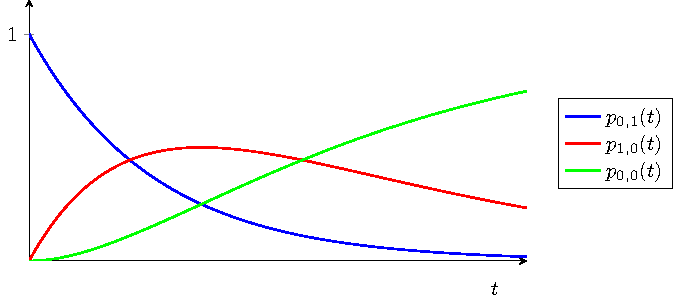
\includegraphics[width=0.66\textwidth]{figures/IMG_ch3/abs2.pdf}
  \caption{State probabilities for the single-particle absorption--death model.
  The particle begins outside, may be absorbed while alive, and eventually reaches
  the dead state.  These three curves are the coefficients of the one-particle
  PGF and sum to one at every time.}
  \label{m:fig:absdeath-state-probabilities}
\end{figure}
Thus the one-particle PGF is
$p_{0,0}+p_{1,0}x+p_{0,1}y$, and independence raises this expression to the
$N$th power, reproducing \cref{m:eq:Gabsdeath}.  At the removable degeneracy
$\alpha=\mu$, l'H\^opital's rule gives
\begin{equation}
  p_{1,0}(t)=\alpha t\ee^{-\alpha t},
  \label{m:eq:absdeath-equal-rates}
\end{equation}
so the stochastic model remains regular even though the separated expression
contains $\mu-\alpha$ in its denominator.

The PGF also recovers the full joint law without another differential equation.
Put $c=p_{0,0}(t)$, $f=p_{1,0}(t)$ and $g=p_{0,1}(t)$.  Since
$G=(c+fx+gy)^N$, coefficient extraction gives
\begin{equation}
  \pr{X_t=i,Y_t=j}
  =\frac{N!}{i!j!(N-i-j)!}
   f^i g^j c^{N-i-j},
  \qquad i+j\leq N.
  \label{m:eq:absdeath-trinomial-law}
\end{equation}
Thus the characteristic solution contains a trinomial distribution over the
three possible single-particle states.  Differentiation at $(x,y)=(1,1)$ gives
\begin{equation}
  \ex{X_t}=Nf(t),
  \qquad
  \ex{Y_t}=Ng(t),
  \qquad
  \operatorname{Cov}(X_t,Y_t)=-Nf(t)g(t).
  \label{m:eq:absdeath-moment-checks}
\end{equation}
The negative covariance records competition between mutually exclusive states of
the same initial particle.  These coefficient and moment checks test more than
normalisation: they confirm that the characteristic inversion has retained the
correct joint dependence.

Several checks now test different parts of the calculation.  At $t=0$ the PGF is
$y^N$; at $x=y=1$ it is one; and its coefficients are non-negative state
probabilities summing to one.  Differentiation verifies the PDE, while the
single-particle calculation verifies the characteristic inversion independently.
The method is useful precisely because the same steps continue to work when birth
opens an infinite interior state space and no finite-state shortcut remains.  The
absorption-only and absorption--birth--death extensions, together with coefficient
recovery, are retained in \cref{m:app:extended-absorption}.

To see the change caused by birth without adding a second worked derivation, let
interior particles reproduce at rate $\lambda$ as well as die at rate $\mu$.
The absorption term is unchanged, but the interior birth transition contributes
$\lambda(x^2-x)G_x$.  The PGF equation is therefore
\begin{equation}
  G_t=\{\lambda x^2-(\lambda+\mu)x+\mu\}G_x
      +\alpha(x-y)G_y.
  \label{m:eq:abd-main-pointer}
\end{equation}
The coefficient of $G_x$ is the same factored birth--death polynomial encountered
in \cref{m:eq:bdpde}.  What changes is the state space: reproduction destroys the
three-state reduction, so the characteristic calculation is no longer merely an
alternative to finite-state independence.  Appendix~\ref{m:app:extended-absorption}
retains the resulting characteristic system, closed form and coefficient-recovery
machinery.  The main text thus supplies one complete worked example while keeping
the extended model available for later use.

\FloatBarrier
